\documentclass{beamer}

\usepackage{lstcustom} 
\usepackage{graphicx}

%\usetheme{Madrid}
\usetheme{Singapore}
%\usetheme{Pittsburgh}

\lstdefinelanguage{Rascal}[]{Java}{
  morekeywords={module, syntax, start, alias, data, visit, top-down, bottom-up, list, str,real},
  moredelim=[is][\textcolor{darkgray}]{\%\%}{\%\%},
  moredelim=[il][\textcolor{darkgray}]{§§}
}

\lstdefinelanguage{FSM}[]{Java}{
  morekeywords={initial, state},
  moredelim=[is][\textcolor{darkgray}]{\%\%}{\%\%},
  moredelim=[il][\textcolor{darkgray}]{§§}
}

\title{Program Analysis and Manipulation Using Rascal}

\author{Rodrigo Bonif\'{a}cio \\ \url{rbonifacio@unb.br}}

\begin{document}

\begin{frame}
\titlepage
\end{frame}

\section{Overview}

\begin{frame}
  \begin{quote}
Rascal is an experimental domain specific language for metaprogramming, such as static code analysis, program transformation and implementation of domain specific languages. It is a general meta language in the sense that it does not have a bias for any particular software language.
  \end{quote}
  \flushright{Wikipedia}
\end{frame}

\begin{frame}
  \begin{block}{Usage scenario}
    Rascal-MPL allows a developer
    to create full-fledged DSLs and program
    analysis and manipulation tools,
    including support for syntax
    definition and strategic programming. 
  \end{block}
\end{frame}

\begin{frame}
  \frametitle{Features}

  \begin{itemize}
    \item hybrid programming model (imperative and functional styles)
    \item immutable data structures and support for generic types
    \item pattern matching and visitors using different strategies
    \item syntax definitions and parsing + REPL support  
    \item Java and Eclipse integration  
  \end{itemize}  
\end{frame}

\begin{frame}
\tableofcontents
\end{frame}

\section{(S1) Lang. Constructs}

\begin{frame}
  \begin{Huge}
    {\color{blue}Section 01:} 
  \end{Huge}

  \vskip+1.5em

  \begin{itemize}
  \item Exploring Rascal Concepts using Colored Trees
  \end{itemize}

\pause
\vskip+5em  
\flushright{\scriptsize{The following slides are based on the P. Klint's Introductory Course on Rascal}}

\end{frame}

\begin{frame}[fragile]

  \begin{columns}
  \begin{column}{0.7\textwidth}
  \begin{small}
  \begin{lstlisting}[language=Rascal]
module ColoredTrees

data ColoredTree = Leaf(int N)
                 | Red(ColoredTree left, ColoredTree right)
                 | Black(ColoredTree left, ColoredTree right)
                 ;


ColoredTree sample = Red(Black(Leaf(1), Red(leaf(2), Leaf(3))),
                     Black(Leaf(4), Leaf(5))); 
  \end{lstlisting}
  \end{small}
  \end{column}
  \begin{column}{0.3\textwidth}
    \begin{center}
      \pause 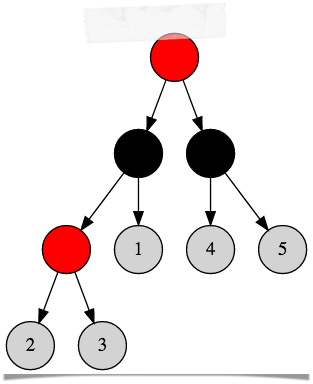
\includegraphics[scale=0.25]{images/rb01.png}
  \end{center}    
  \end{column}
  \end{columns}
  
\end{frame}

\begin{frame}[fragile]
  \frametitle{Pattern Matching (switch-case)}

    \begin{small}
      \begin{lstlisting}[language=Rascal]
// number of nodes  
int elements(ColoredTree tree) {
  switch(tree) {
    case Leaf(n) : return 1; 
    case Black(l, r): return 1 + elements(l) + elements(r);
    case Red(l, r) : return 1 + elements(l) + elements(r);
  }
  return res; 
} 
\end{lstlisting}
    \end{small}

  
\end{frame}

\begin{frame}[fragile]
  \frametitle{Pattern Matching (visitor to collect information)}

    \begin{small}
      \begin{lstlisting}[language=Rascal]
    // total of values in a tree (imperative style)     
    int sumTree(ColoredTree tree) {
      int res = 0;
      top-down visit (tree) {
        case Leaf(n): res = res + n;
      }
      return res;
    }
\end{lstlisting}
\end{small}

  \begin{itemize}
    \item Traversal strategies
      \begin{itemize}
        \item top-down visit (top-down-break)
        \item bottom-up visit (bottom-up-break)
        \item innermost
        \item outermost  
      \end{itemize}  
  \end{itemize}  
\end{frame}

\begin{frame}[fragile]
  \frametitle{Pattern Matching (visitor to transform a tree)}

  \begin{lstlisting}[language=Rascal]
    // increment all values in a tree 
    ColoredTree increment(ColoredTree tree) =
      top-down visit (tree) {
        case Leaf(n) => leaf(n + 1)
      };
    \end{lstlisting}  
  \pause

  \begin{block}{Change all reds to green}
    \begin{lstlisting}[language=Rascal]
    data ColoredTree = Green(ColoredTree l, ColoredTree r);   
    ColoredTree allRedsToGreen(ColoredTree tree) =
      top-down-break visit (tree) {
        case Red(l, r) => Green(l, r)
      };
    \end{lstlisting}  
  \end{block}
\end{frame}

\begin{frame}
  \centering{
    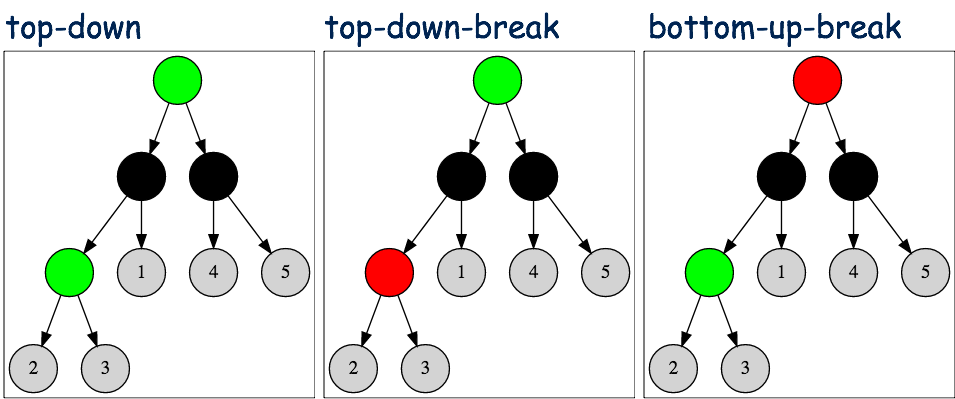
\includegraphics[scale=0.3]{images/visitors.png}
  }
\end{frame}

\begin{frame}[fragile]
  \frametitle{Comprehension}

  \begin{small}
  \begin{verbatim}
    GHCi, version 7.10.3: http://www.haskell.org/ghc/  :? for help
    Prelude> let list = [1..10]
    Prelude> [x * x | x <- list, even x]
    [4,16,36,64,100]    
  \end{verbatim}\end{small} \pause
  
  Comprehension is available in many programming languages\pause,
  including Haskell, Python, Rascal, and so on. \pause 

  \begin{block}{Rascal goes further, combining comprehension and generic traversals}
   \begin{lstlisting}[language=Rascal]
     rascal> [n | /leaf(int n) <- sample()];
     list[int]: [1,2,3,4,5]
   \end{lstlisting}
  \end{block}
  
\end{frame}

\begin{frame}
  \begin{block}{Exercise 01}
    \begin{itemize}
      \item implement a function that converts only the top-level \texttt{red} nodes into \texttt{green} nodes
        \item re-implement \texttt{elements} and \texttt{sumTree} using a more {\color{blue}functional style}   
    \end{itemize}
  \end{block}  
\end{frame}
\begin{frame}[fragile]
  \frametitle{String Interpolation: Export to DOT Notation (1/3)}

    \begin{lstlisting}[language=Rascal]
    str export(ColoredTree t) {
      str g = "digraph g { \n";
        int id = 0;
        map[ColoredTree, str] decls = ();
\end{lstlisting}

\end{frame}

\begin{frame}[fragile]
  \frametitle{String Interpolation: Export to DOT Notation (2/3)}

  \begin{small}
    \begin{lstlisting}[language=Rascal]
        // print the nodes
        top-down visit(t) {
          case red(l, r) :
          {
            id = id + 1;
            g += "  n<id> [label = \"\" shape = circle fillcolor = red style = filled]\n";
            decls += (red(l,r) : "n<id>");
          }
          case black(l, r) :
          {
            id = id + 1;
            g += "  n<id> [label = \"\" shape = circle fillcolor = black style = filled]\n";
            decls += (black(l,r) : "n<id>");
          }
          case leaf(n) :
          {
            id = id + 1;
            g = g + "  n<id> [label = <n>] \n";
            decls += (leaf(n) : "n<id>");
          }
        };
\end{lstlisting}
  \end{small}
\end{frame}

\begin{frame}[fragile]
  \frametitle{String Interpolation: Export to DOT Notation (3/3)}
  \begin{small}
    \begin{lstlisting}[language=Rascal]
        // print the edges
        top-down visit(t) {
          case red(l, r) : {
            g += "  <decls[red(l,r)]> -\> <decls[l]> \n";
            g += "  <decls[red(l,r)]> -\> <decls[r]> \n";
          }
          case black(l, r) : {
            g += "  <decls[black(l,r)]> -\> <decls[l]> \n";
            g += "  <decls[black(l,r)]> -\> <decls[r]> \n";
          }
        }

        g += "}";

      return g;
    }
  \end{lstlisting}  
  \end{small}  
\end{frame}

\section{(S2) Hands On}

\begin{frame}
  \begin{huge}
    {\color{blue}Section 02:}
  \end{huge}  
  \vskip1.5em

  \begin{itemize}
    \item Hands on: Scrap Your Boilerplate
  \end{itemize}
\end{frame}
\begin{frame}
  
\begin{center}
 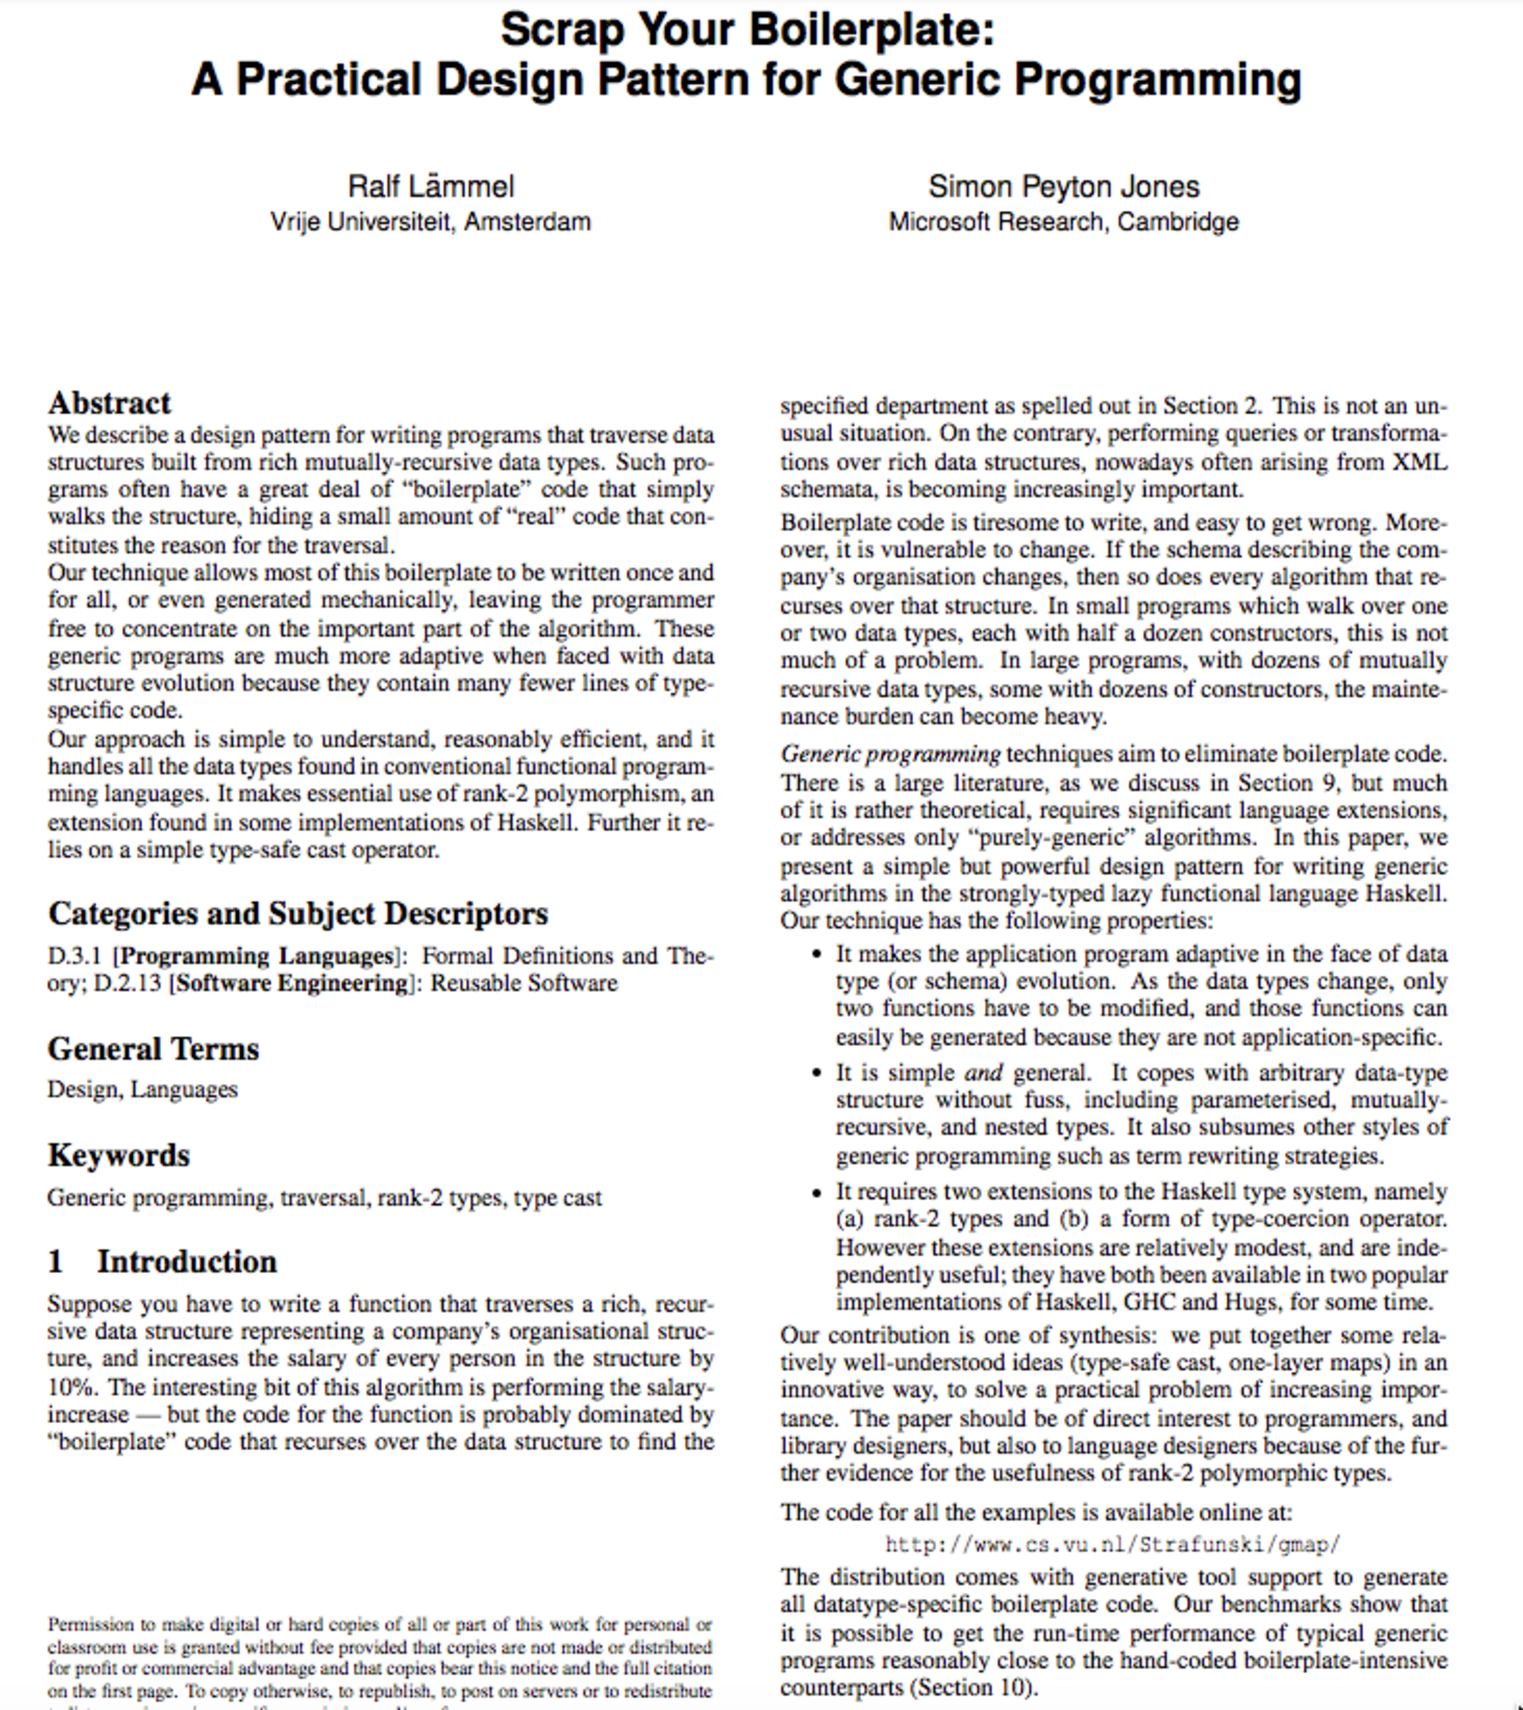
\includegraphics[scale=0.3]{images/syb-paper.pdf}
\end{center}
\end{frame}

\begin{frame}
  \frametitle{Problem: generic traversals}

  \begin{center}
    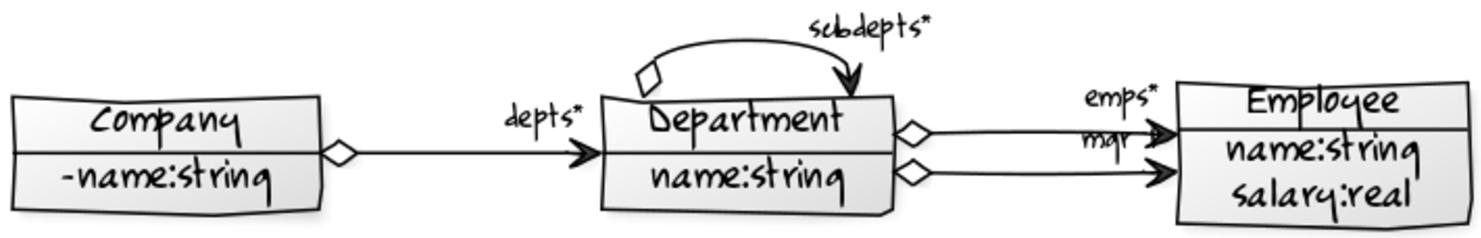
\includegraphics[scale=0.4]{images/dm.pdf}
  \end{center}

  \pause \vskip+1.5em

  \begin{block}{Programming task \ldots}
    \begin{itemize}
    \item compute the total of salaries in a company
    \item cut the salaries of a company by a given percentage
    \end{itemize}  
  \end{block}
\end{frame}

\begin{frame}[fragile]
  \frametitle{Domain model in Haskell}

  \begin{lstlisting}[language=Haskell]
module Companies where 

type Name    = String
type Salary  = Double
type Manager = Employee 

data Company    = C Name [Department]
data Department = D Name Manager [Department] [Employee]
data Employee   = E Name Salary

  \end{lstlisting}  
\end{frame}

\begin{frame}[fragile]
  \frametitle{Cutting salaries in Haskell}

  \begin{lstlisting}[language=Haskell]
cut :: Double -> Company -> Company
cut k (C n depts) = C n (map (cutD k) depts)

cutD :: Double -> Department -> Department
cutD k (D n mgr subdepts emps) = D n (cutE k mgr) (map (cutD k) subdepts) (map (cutE k) emps)

cutE :: Double -> Employee -> Employee
cutE k (E n s) = E n (s - (k * s)) 
  \end{lstlisting}  
\end{frame}

\begin{frame}[fragile]
  \frametitle{Total salaries in Haskell}

  \begin{lstlisting}[language=Haskell]
total :: Company -> Salary
total (C _ depts) = sum (map totalD depts)

totalD :: Department -> Salary
totalD (D _ mgr subdepts emps) = salary mgr
                               + sum (map totalD subdepts)
			       + sum (map salary emps)

salary :: Employee -> Salary
salary (E _ s) = s

  \end{lstlisting} 
\end{frame}

\begin{frame}
 \huge{Let's implement this problem using Rascal-MPL}
\end{frame}


\begin{frame}[fragile]
  \frametitle{Domain Model}

  \begin{lstlisting}[language=Rascal]
alias Name    = str;
alias Salary  = real; 
alias Manager = Employee; 

data Company = company(Name n, list[Department] deps); 
data Department = department(Name name, Manager mgr, list[Department] subdeps, list[Employee] emps); 
data Employee = employee(Name name, Salary salary); 
  \end{lstlisting}  
\end{frame}

\begin{frame}[fragile]
  \frametitle{Test Cases}

  \begin{lstlisting}
Employee ralf = employee("ralf", 8000.0); 
Employee joost = employee("joost", 1000.0);
Employee marlow = employee("marlow", 2000.0);
Employee blair = employee("blair", 100000.0);

Department research = department("research", ralf, [], [joost, marlow]); 
Department strategy = department("strategy", blair, [], []); 

public Company genCom = company("genCom", [research, strategy]);

test bool testTotal() = 111000.0 == total(genCom);

test bool testIncrease() = 122100.0 == increase(0.1, genCom);
  \end{lstlisting}
\end{frame}

\begin{frame}
 \begin{center} 
   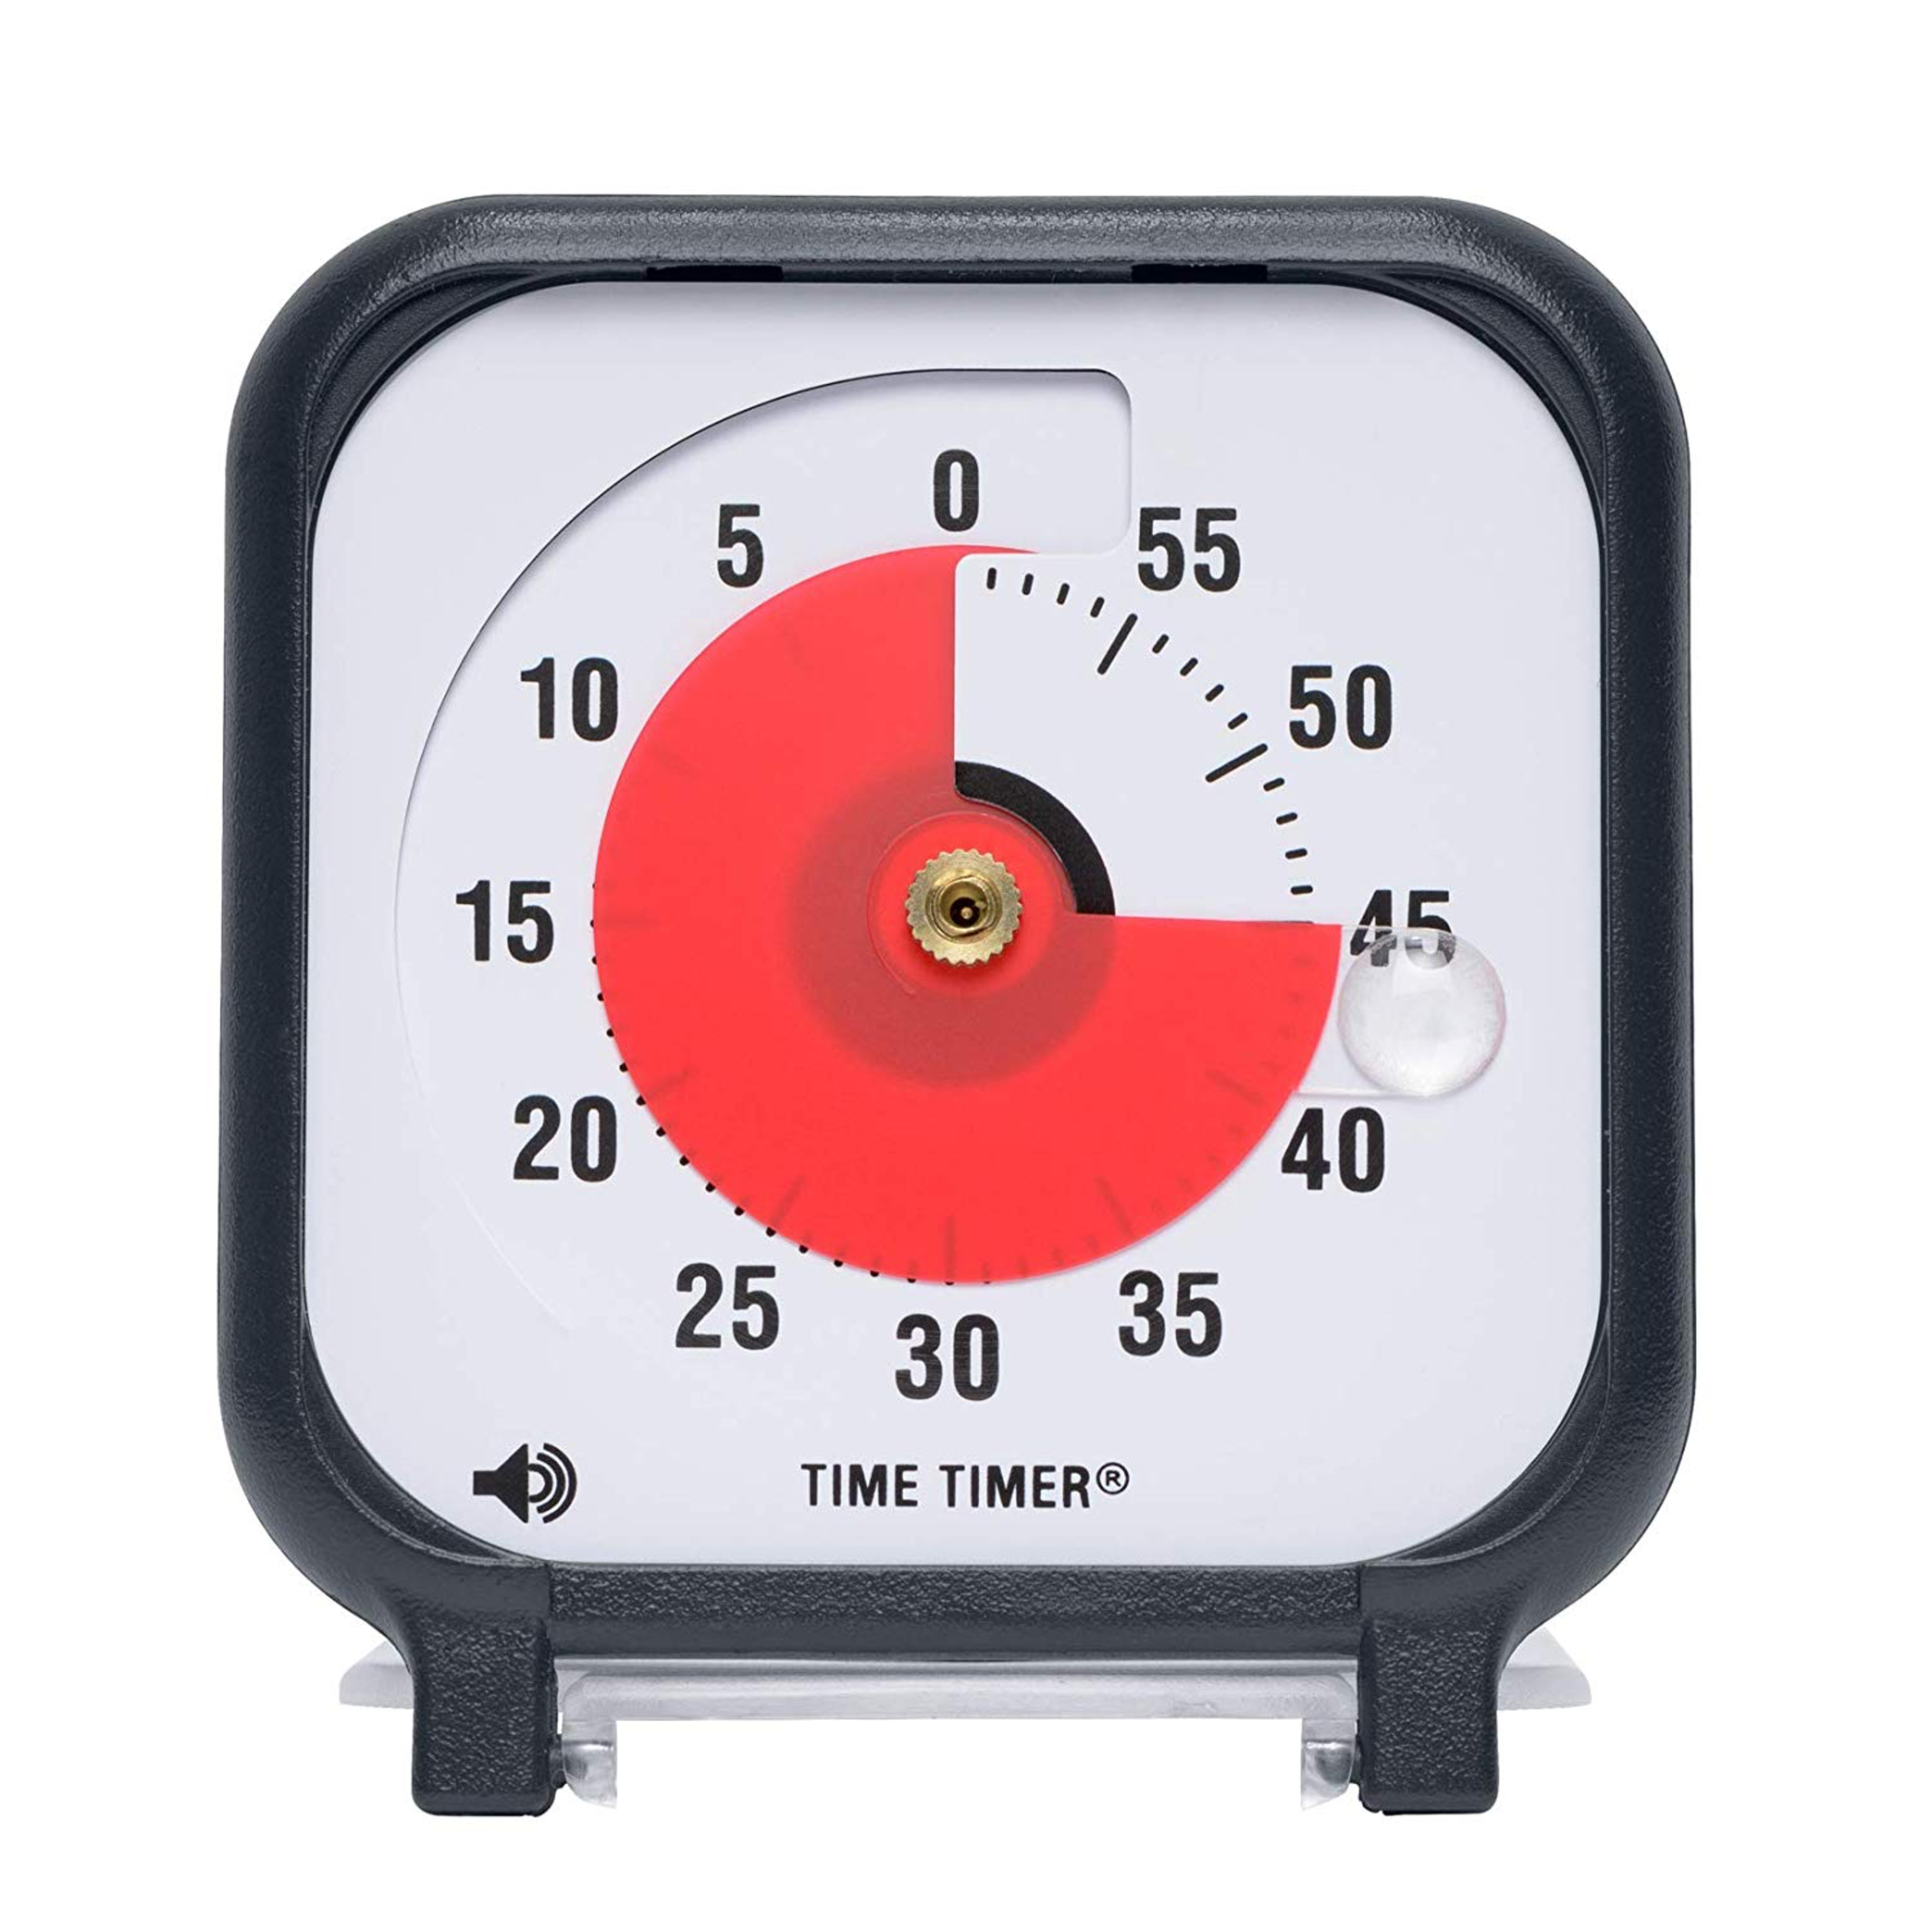
\includegraphics[scale=0.15]{images/timer.pdf}
 \end{center}   
\end{frame}

\begin{frame}
  \begin{block}{Exercise 02}
    Implement the following functions:

    \begin{itemize}
      \item increase the salary of all managers
      \item find the highest salary of a company
      \item find the salary of a given employee
    \end{itemize}
  \end{block}  
\end{frame}

\section{(S3) Parsing}

\begin{frame}
  \begin{huge}
    {\color{blue}Section 03:} 
  \end{huge}
  \vskip+1.5em
  \begin{itemize}
    \item Exploring Syntax Definition, Parsing, and
    Pattern Matching on Concrete Syntax
  \end{itemize}
\end{frame}

\begin{frame}
  \frametitle{Syntax Definition}

  \begin{itemize}
  \item converts a grammar into a parser
  \item main components (context free grammar) 
    \begin{itemize}
    \item syntax expressed using production rules
    \item lexical, layout, and keyword definitions
    \end{itemize} \pause
  \item challenge: disambiguation
  \end{itemize}

\end{frame}

\begin{frame}[fragile]
\frametitle{Let's consider a language for FSMs} 

\begin{lstlisting}[language=Rascal]
module lang::fsm::AbstractSyntax

data StateMachine 
  = fsm(list[State] states, list[Transition] transitions);

data State 
  = state(str name)
  | startState(str name)
  ;
           
data Transition 
  = transition(str source, Event event, str target);
  
data Event 
  = event(str evt)
  | eventWithAction(str evt, str action)
  ;
\end{lstlisting}
\end{frame}

\begin{frame}[fragile]
 \frametitle{Example of a FSM specification}

 \begin{lstlisting}[language=FSM]
initial state locked {
  ticket/collect -> unlocked;
  pass/alarm -> exception;
}

state unlocked {
  ticket/eject;
  pass -> locked;
}

state exception {
  ticket/eject;
  pass;
  mute;
  release -> locked;
}
 \end{lstlisting}
\end{frame}

\begin{frame}[fragile]
\frametitle{A grammar definition for FSMs using Rascal}

\begin{lstlisting}[language=Rascal]
module lang::fsm::ConcreteSyntax

start syntax FSM = CState* states;

syntax CState 
  = initialState: "initial" "state" Id "{" CEvent* "}"
  | basicState: "state" Id "{" CEvent* "}"
  ;

syntax CEvent 
  = basicEvent: Id ("-\>" Id)? ";"
  | actionEvent: Id "/" Id ("-\>" Id)? ";"
  ; 

lexical Id = [a-zA-Z][_a-zA-Z0-9]*; 

lexical Comment = "//" ![\n]* [\n];

lexical Spaces = [\n\r\f\t\ ]*;

layout Layout = Spaces 
              | Comment 
              ; 

keyword Keywords = "state" | "initial" ;
\end{lstlisting} 

\end{frame}

\begin{frame}[fragile]
\frametitle{A parser from Concrete Syntax to Abstract Syntax (1/2)}

\begin{lstlisting}[language=Rascal]
module lang::fsm::Parser

import ParseTree;
import IO;

import lang::fsm::ConcreteSyntax;
import lang::fsm::AbstractSyntax; 

public StateMachine parseFSM(str f) {
 loc file = |file:///| + f;
 list[State] states = [];
 list[Transition] transitions = [];
 
 start[FSM] parseResult = parse(#start[FSM], file);
 
 top-down visit (parseResult) {
    case (CState)`initial state <Id id> { <CEvent* evts>}`: {
      states += startState(unparse(id));
      transitions += parseEvents(id, evts);
    }
    case (CState)`state <Id id> { <CEvent* evts>}`: {
      states += state(unparse(id));
      transitions += parseEvents(id, evts);
    }
 };
 
 return fsm(states, transitions);
}
\end{lstlisting}

\end{frame}

\begin{frame}[fragile]
\frametitle{A parser from Concrete Syntax to Abstract Syntax (2/2)}

\begin{lstlisting}[language=Rascal]
list[Transition] parseEvents(Id source, CEvent* evts) {
  list[Transition] ts = [];
  top-down visit(evts) {
    case (CEvent)`<Id e> -\> <Id target>;` : 
      ts += transition(unparse(source), event(unparse(e)), unparse(target));
    case (CEvent)`<Id e>;` : 
      ts += transition(unparse(source), event(unparse(e)), unparse(source));
    case (CEvent)`<Id e> / <Id a> -\> <Id target>;` : 
      ts += transition(unparse(source), eventWithAction(unparse(e), unparse(a)), unparse(target));
    case (CEvent)`<Id e> / <Id a>;` : 
      ts += transition(unparse(source), eventWithAction(unparse(e), unparse(a)), unparse(source));
  }
  return ts;
}
\end{lstlisting}

\end{frame}

\begin{frame}

  \begin{block}{Exercise 03}
    Implement the following functions on FSMs
    \begin{itemize}
      \item interpretation, code generation, and visualization
      \item wfr: single start state, deterministic transitions, reachable states
    \end{itemize}
  \end{block}
\end{frame}

\section{(S4) SCAM}

\begin{frame}
  \begin{huge}
    Section 04:
  \end{huge}

  \vskip+1.5em
\begin{block}{Program Analysis and Manipulation}
  \begin{itemize}
    \item Counting atoms of confusion in source code
    \item Estimating cyclomatic complexity of methods 
    \item Transforming Java Code (RJTL,SpongeBugs)\footnote{[SANER2018, SBES2019, SCAM2019]}
  \end{itemize}
  \end{block}
\end{frame}

\begin{frame}[fragile]
  \frametitle{Counting atoms of confusion (using concrete syntax)}

  \begin{lstlisting}[language=Rascal]
void analyse(CompilationUnit unit) {
  top-down visit(unit) {
    case (Expression)`<OctaNumeral n>`:
      recordAtom("LiteralEncoding"); 

    case (Expression)`<Identifier id>++`:
      recordAtom("PostIncrement");

    case (Expression)`++<Identifier id>`:
      recordAtom("PreIncrement"); 

    case (Expression)`<ConditionalOrExpression e> ? <Expression e1> : <ConditionalExpression e>`:
      recordAtom("ConditionalOperator");

    // ... 
  }
}
  \end{lstlisting}  
\end{frame}

\begin{frame}[fragile]
  \begin{block}{The \texttt{main} program}

    \begin{lstlisting}[language=Rascal]
map[str, int] atoms = ();

public void execute(loc srcdir) {
  files = findAllFiles(srcdir, "java");
  real errors = 0.0; 
  for(f <- files) {
    try { 
      CompilationUnit unit = parse(#CompilationUnit, f); 
      analyse(unit);
    }
    catch e: {
      errors += 1;
    }
  }
	
  for(k <- atoms) {
    println("<k> : <atoms[k]>"); 
  }
	
  totalFiles = size(files);
  println("Could not parse <errors> files (<errors * 100.0 / totalFiles> %)"); 
}
    \end{lstlisting}
    \end{block}
\end{frame}

\begin{frame}[fragile]
\begin{small}
\begin{verbatim}
rascal>import analysis::AtomsOfConfusion;
ok
rascal>execute(|project://atoms/sample/lucene-core/|);
LiteralEncoding : 1
ConditionalOperator : 714
PreIncrement : 40
PostIncrement : 3291

Could not parse 10.0 files (0.71% of all files)  
\end{verbatim}
\end{small}
\end{frame}

\begin{frame}[fragile]
  \frametitle{Cyclomatic Complexity}

  \begin{lstlisting}[language=Rascal]
void recordCC(Identifier id, MethodBody b) { 
  int total = 1;
  top-down visit(b) {
    case (Statement)`if(<Expression c>) <Statement s>` : total += 1; 
    case (Statement)`if(<Expression c>) <StatementNoShortIf s1> else <Statement s2>` : total += 1; 
    case (Statement)`while(<Expression c>) <Statement s>` : total += 1; 
    case (Statement)`for(<ForInit init>; <Expression e1>; <StatementExpressionList e2>) <Statement s>` : total += 1;
    case (SwitchLabel)`case <Expression e>:` : total += 1; 
    case (SwitchLabel)`default :` : total +=1;  
  }
  cc += (unparse(id) : total); 
}
  \end{lstlisting}
\end{frame}

\begin{frame}[fragile]
  \frametitle{Anonymous Inner Classes to Lambda Expressions}

  \begin{lstlisting}[language=Rascal]
public CompilationUnit aicToLambda(CompilationUnit unit) {
  list[ImportClause] imports = listOfImports(unit);
  CompilationUnit res = visit(unit) {
    case (Expression)`new <ClassOrInterfaceTypeToInstantiate id>() {
                     '   <MethodModifier m> <Result res> <Identifier methodName> () {
                     '     <Statement stmt>
                     '   }
                     ' }` => (Expression)`()-\> { <Statement stmt >}` 
       when checkConstraints(stmt, methodName, imports)   
  }
  return res;
}
\end{lstlisting}
\end{frame}

\begin{frame}
  \begin{block}{Exercise 04:}
    \begin{itemize}
      \item Implement new constraints on RJTL transformations
      \item Project: rewrite the C grammar of Rascal to support pre-processor directives \pause
        and analyse C code!
    \end{itemize}  
  \end{block}  
\end{frame}

\section{(S5) Final Remarks}

\begin{frame}
  \begin{huge}
    Section 05: 
  \end{huge}

  \vskip+1.5em
  Final Remarks \ldots 
\end{frame}

\begin{frame}
  \begin{itemize}
   \item Rascal is a powerful language for program analysis and manipulation \pause 
   \item Deciding how to combine the imperative and functional styles is challenging \pause 
   \item Some analysis and transformations are difficult to implement considering only the source code \end{itemize}
\end{frame}

\begin{frame}
  

  \begin{huge}Thanks\end{huge}

    \pause
    \vskip+1.5em

    \begin{block}{Directions}
     \begin{scriptsize}
     \begin{itemize}
       \item http://www.rascal-mpl.org/
       \item http://tutor.rascal-mpl.org/
       \item https://github.com/rbonifacio/rascal-course-cbsoft
       \item https://github.com/refactoring-towards-language-evolution/rascal-Java8
       \item https://github.com/dvmarcilio/SpongeBugs  
     \end{itemize}
     \end{scriptsize}
   \end{block}

\end{frame}

\end{document}
